\documentclass[1p]{elsarticle_modified}
%\bibliographystyle{elsarticle-num}

%\usepackage[colorlinks]{hyperref}
%\usepackage{abbrmath_seonhwa} %\Abb, \Ascr, \Acal ,\Abf, \Afrak
\usepackage{amsfonts}
\usepackage{amssymb}
\usepackage{amsmath}
\usepackage{amsthm}
\usepackage{scalefnt}
\usepackage{amsbsy}
\usepackage{kotex}
\usepackage{caption}
\usepackage{subfig}
\usepackage{color}
\usepackage{graphicx}
\usepackage{xcolor} %% white, black, red, green, blue, cyan, magenta, yellow
\usepackage{float}
\usepackage{setspace}
\usepackage{hyperref}

\usepackage{tikz}
\usetikzlibrary{arrows}

\usepackage{multirow}
\usepackage{array} % fixed length table
\usepackage{hhline}

%%%%%%%%%%%%%%%%%%%%%
\makeatletter
\renewcommand*\env@matrix[1][\arraystretch]{%
	\edef\arraystretch{#1}%
	\hskip -\arraycolsep
	\let\@ifnextchar\new@ifnextchar
	\array{*\c@MaxMatrixCols c}}
\makeatother %https://tex.stackexchange.com/questions/14071/how-can-i-increase-the-line-spacing-in-a-matrix
%%%%%%%%%%%%%%%

\usepackage[normalem]{ulem}

\newcommand{\msout}[1]{\ifmmode\text{\sout{\ensuremath{#1}}}\else\sout{#1}\fi}
%SOURCE: \msout is \stkout macro in https://tex.stackexchange.com/questions/20609/strikeout-in-math-mode

\newcommand{\cancel}[1]{
	\ifmmode
	{\color{red}\msout{#1}}
	\else
	{\color{red}\sout{#1}}
	\fi
}

\newcommand{\add}[1]{
	{\color{blue}\uwave{#1}}
}

\newcommand{\replace}[2]{
	\ifmmode
	{\color{red}\msout{#1}}{\color{blue}\uwave{#2}}
	\else
	{\color{red}\sout{#1}}{\color{blue}\uwave{#2}}
	\fi
}

\newcommand{\Sol}{\mathcal{S}} %segment
\newcommand{\D}{D} %diagram
\newcommand{\A}{\mathcal{A}} %arc


%%%%%%%%%%%%%%%%%%%%%%%%%%%%%5 test

\def\sl{\operatorname{\textup{SL}}(2,\Cbb)}
\def\psl{\operatorname{\textup{PSL}}(2,\Cbb)}
\def\quan{\mkern 1mu \triangleright \mkern 1mu}

\theoremstyle{definition}
\newtheorem{thm}{Theorem}[section]
\newtheorem{prop}[thm]{Proposition}
\newtheorem{lem}[thm]{Lemma}
\newtheorem{ques}[thm]{Question}
\newtheorem{cor}[thm]{Corollary}
\newtheorem{defn}[thm]{Definition}
\newtheorem{exam}[thm]{Example}
\newtheorem{rmk}[thm]{Remark}
\newtheorem{alg}[thm]{Algorithm}

\newcommand{\I}{\sqrt{-1}}
\begin{document}

%\begin{frontmatter}
%
%\title{Boundary parabolic representations of knots up to 8 crossings}
%
%%% Group authors per affiliation:
%\author{Yunhi Cho} 
%\address{Department of Mathematics, University of Seoul, Seoul, Korea}
%\ead{yhcho@uos.ac.kr}
%
%
%\author{Seonhwa Kim} %\fnref{s_kim}}
%\address{Center for Geometry and Physics, Institute for Basic Science, Pohang, 37673, Korea}
%\ead{ryeona17@ibs.re.kr}
%
%\author{Hyuk Kim}
%\address{Department of Mathematical Sciences, Seoul National University, Seoul 08826, Korea}
%\ead{hyukkim@snu.ac.kr}
%
%\author{Seokbeom Yoon}
%\address{Department of Mathematical Sciences, Seoul National University, Seoul, 08826,  Korea}
%\ead{sbyoon15@snu.ac.kr}
%
%\begin{abstract}
%We find all boundary parabolic representation of knots up to 8 crossings.
%
%\end{abstract}
%\begin{keyword}
%    \MSC[2010] 57M25 
%\end{keyword}
%
%\end{frontmatter}

%\linenumbers
%\tableofcontents
%
\newcommand\colored[1]{\textcolor{white}{\rule[-0.35ex]{0.8em}{1.4ex}}\kern-0.8em\color{red} #1}%
%\newcommand\colored[1]{\textcolor{white}{ #1}\kern-2.17ex	\textcolor{white}{ #1}\kern-1.81ex	\textcolor{white}{ #1}\kern-2.15ex\color{red}#1	}

{\Large $\underline{12n_{0854}~(K12n_{0854})}$}

\setlength{\tabcolsep}{10pt}
\renewcommand{\arraystretch}{1.6}
\vspace{1cm}\begin{tabular}{m{100pt}>{\centering\arraybackslash}m{274pt}}
\multirow{5}{120pt}{
	\centering
	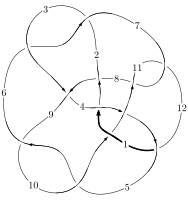
\includegraphics[width=112pt]{../../../GIT/diagram.site/Diagrams/png/2943_12n_0854.png}\\
\ \ \ A knot diagram\footnotemark}&
\allowdisplaybreaks
\textbf{Linearized knot diagam} \\
\cline{2-2}
 &
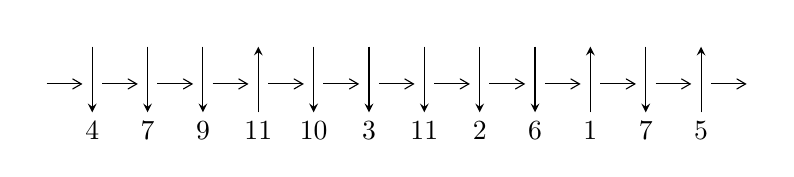
\begin{tikzpicture}[x=20pt, y=17pt]
	% nodes
	\node (C0) at (0, 0) {};
	\node (C1) at (1, 0) {};
	\node (C1U) at (1, +1) {};
	\node (C1D) at (1, -1) {4};

	\node (C2) at (2, 0) {};
	\node (C2U) at (2, +1) {};
	\node (C2D) at (2, -1) {7};

	\node (C3) at (3, 0) {};
	\node (C3U) at (3, +1) {};
	\node (C3D) at (3, -1) {9};

	\node (C4) at (4, 0) {};
	\node (C4U) at (4, +1) {};
	\node (C4D) at (4, -1) {11};

	\node (C5) at (5, 0) {};
	\node (C5U) at (5, +1) {};
	\node (C5D) at (5, -1) {10};

	\node (C6) at (6, 0) {};
	\node (C6U) at (6, +1) {};
	\node (C6D) at (6, -1) {3};

	\node (C7) at (7, 0) {};
	\node (C7U) at (7, +1) {};
	\node (C7D) at (7, -1) {11};

	\node (C8) at (8, 0) {};
	\node (C8U) at (8, +1) {};
	\node (C8D) at (8, -1) {2};

	\node (C9) at (9, 0) {};
	\node (C9U) at (9, +1) {};
	\node (C9D) at (9, -1) {6};

	\node (C10) at (10, 0) {};
	\node (C10U) at (10, +1) {};
	\node (C10D) at (10, -1) {1};

	\node (C11) at (11, 0) {};
	\node (C11U) at (11, +1) {};
	\node (C11D) at (11, -1) {7};

	\node (C12) at (12, 0) {};
	\node (C12U) at (12, +1) {};
	\node (C12D) at (12, -1) {5};
	\node (C13) at (13, 0) {};

	% arrows
	\draw[->,>={angle 60}]
	(C0) edge (C1) (C1) edge (C2) (C2) edge (C3) (C3) edge (C4) (C4) edge (C5) (C5) edge (C6) (C6) edge (C7) (C7) edge (C8) (C8) edge (C9) (C9) edge (C10) (C10) edge (C11) (C11) edge (C12) (C12) edge (C13) ;	\draw[->,>=stealth]
	(C1U) edge (C1D) (C2U) edge (C2D) (C3U) edge (C3D) (C4D) edge (C4U) (C5U) edge (C5D) (C6U) edge (C6D) (C7U) edge (C7D) (C8U) edge (C8D) (C9U) edge (C9D) (C10D) edge (C10U) (C11U) edge (C11D) (C12D) edge (C12U) ;
	\end{tikzpicture} \\
\hhline{~~} \\& 
\textbf{Solving Sequence} \\ \cline{2-2} 
 &
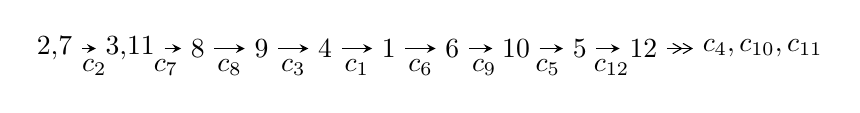
\begin{tikzpicture}[x=23pt, y=7pt]
	% node
	\node (A0) at (-1/8, 0) {2,7};
	\node (A1) at (17/16, 0) {3,11};
	\node (A2) at (17/8, 0) {8};
	\node (A3) at (25/8, 0) {9};
	\node (A4) at (33/8, 0) {4};
	\node (A5) at (41/8, 0) {1};
	\node (A6) at (49/8, 0) {6};
	\node (A7) at (57/8, 0) {10};
	\node (A8) at (65/8, 0) {5};
	\node (A9) at (73/8, 0) {12};
	\node (C1) at (1/2, -1) {$c_{2}$};
	\node (C2) at (13/8, -1) {$c_{7}$};
	\node (C3) at (21/8, -1) {$c_{8}$};
	\node (C4) at (29/8, -1) {$c_{3}$};
	\node (C5) at (37/8, -1) {$c_{1}$};
	\node (C6) at (45/8, -1) {$c_{6}$};
	\node (C7) at (53/8, -1) {$c_{9}$};
	\node (C8) at (61/8, -1) {$c_{5}$};
	\node (C9) at (69/8, -1) {$c_{12}$};
	\node (A10) at (11, 0) {$c_{4},c_{10},c_{11}$};

	% edge
	\draw[->,>=stealth]	
	(A0) edge (A1) (A1) edge (A2) (A2) edge (A3) (A3) edge (A4) (A4) edge (A5) (A5) edge (A6) (A6) edge (A7) (A7) edge (A8) (A8) edge (A9) ;
	\draw[->>,>={angle 60}]	
	(A9) edge (A10);
\end{tikzpicture} \\ 

\end{tabular} \\

\footnotetext{
The image of knot diagram is generated by the software ``\textbf{Draw programme}" developed by Andrew Bartholomew(\url{http://www.layer8.co.uk/maths/draw/index.htm\#Running-draw}), where we modified some parts for our purpose(\url{https://github.com/CATsTAILs/LinksPainter}).
}\phantom \\ \newline 
\centering \textbf{Ideals for irreducible components\footnotemark of $X_{\text{par}}$} 
 
\begin{align*}
I^u_{1}&=\langle 
8.39823\times10^{498} u^{108}+2.41008\times10^{499} u^{107}+\cdots+7.17600\times10^{500} b-4.55608\times10^{504},\\
\phantom{I^u_{1}}&\phantom{= \langle  }7.81238\times10^{505} u^{108}+1.77615\times10^{506} u^{107}+\cdots+2.83788\times10^{507} a-3.55368\times10^{511},\\
\phantom{I^u_{1}}&\phantom{= \langle  }u^{109}+36 u^{107}+\cdots-1154036 u-171943\rangle \\
I^u_{2}&=\langle 
2.24797\times10^{42} u^{37}+1.61524\times10^{42} u^{36}+\cdots+1.01090\times10^{43} b-7.15951\times10^{42},\\
\phantom{I^u_{2}}&\phantom{= \langle  }-3.29889\times10^{42} u^{37}-5.18067\times10^{42} u^{36}+\cdots+7.07629\times10^{43} a+2.71417\times10^{43},\;u^{38}+u^{37}+\cdots+8 u+7\rangle \\
\\
\end{align*}
\raggedright * 2 irreducible components of $\dim_{\mathbb{C}}=0$, with total 147 representations.\\
\footnotetext{All coefficients of polynomials are rational numbers. But the coefficients are sometimes approximated in decimal forms when there is not enough margin.}
\newpage
\renewcommand{\arraystretch}{1}
\centering \section*{I. $I^u_{1}= \langle 8.40\times10^{498} u^{108}+2.41\times10^{499} u^{107}+\cdots+7.18\times10^{500} b-4.56\times10^{504},\;7.81\times10^{505} u^{108}+1.78\times10^{506} u^{107}+\cdots+2.84\times10^{507} a-3.55\times10^{511},\;u^{109}+36 u^{107}+\cdots-1154036 u-171943 \rangle$}
\flushleft \textbf{(i) Arc colorings}\\
\begin{tabular}{m{7pt} m{180pt} m{7pt} m{180pt} }
\flushright $a_{2}=$&$\begin{pmatrix}1\\0\end{pmatrix}$ \\
\flushright $a_{7}=$&$\begin{pmatrix}0\\u\end{pmatrix}$ \\
\flushright $a_{3}=$&$\begin{pmatrix}1\\u^2\end{pmatrix}$ \\
\flushright $a_{11}=$&$\begin{pmatrix}-0.0275289 u^{108}-0.0625870 u^{107}+\cdots+82142.5 u+12522.3\\-0.0117032 u^{108}-0.0335853 u^{107}+\cdots+41138.1 u+6349.05\end{pmatrix}$ \\
\flushright $a_{8}=$&$\begin{pmatrix}-0.0285405 u^{108}+0.0104270 u^{107}+\cdots+11834.6 u+1173.41\\0.00263481 u^{108}+0.0158836 u^{107}+\cdots-18487.5 u-2914.67\end{pmatrix}$ \\
\flushright $a_{9}=$&$\begin{pmatrix}-0.0311753 u^{108}-0.00545660 u^{107}+\cdots+30322.1 u+4088.08\\0.00263481 u^{108}+0.0158836 u^{107}+\cdots-18487.5 u-2914.67\end{pmatrix}$ \\
\flushright $a_{4}=$&$\begin{pmatrix}-0.0169095 u^{108}-0.131078 u^{107}+\cdots+144204. u+22938.7\\-0.0147313 u^{108}+0.0146839 u^{107}+\cdots-7112.82 u-1533.36\end{pmatrix}$ \\
\flushright $a_{1}=$&$\begin{pmatrix}0.0444190 u^{108}-0.0696387 u^{107}+\cdots+34828.4 u+6920.06\\-0.0314214 u^{108}+0.0150164 u^{107}+\cdots+9958.32 u+770.043\end{pmatrix}$ \\
\flushright $a_{6}=$&$\begin{pmatrix}u\\u^3+u\end{pmatrix}$ \\
\flushright $a_{10}=$&$\begin{pmatrix}-0.0124119 u^{108}+0.0237295 u^{107}+\cdots-13201.6 u-2454.64\\-0.0143619 u^{108}+0.0345235 u^{107}+\cdots-25103.0 u-4439.04\end{pmatrix}$ \\
\flushright $a_{5}=$&$\begin{pmatrix}-0.0342753 u^{108}-0.0523315 u^{107}+\cdots+77734.8 u+11680.1\\-0.00772236 u^{108}+0.0156642 u^{107}+\cdots-10128.1 u-1906.46\end{pmatrix}$ \\
\flushright $a_{12}=$&$\begin{pmatrix}0.0275289 u^{108}+0.0625870 u^{107}+\cdots-82142.5 u-12522.3\\-0.0520561 u^{108}+0.00229324 u^{107}+\cdots+35822.9 u+4412.34\end{pmatrix}$\\&\end{tabular}
\flushleft \textbf{(ii) Obstruction class $= -1$}\\~\\
\flushleft \textbf{(iii) Cusp Shapes $= 0.216975 u^{108}-0.110555 u^{107}+\cdots-47146.8 u-2137.91$}\\~\\
\newpage\renewcommand{\arraystretch}{1}
\flushleft \textbf{(iv) u-Polynomials at the component}\newline \\
\begin{tabular}{m{50pt}|m{274pt}}
Crossings & \hspace{64pt}u-Polynomials at each crossing \\
\hline $$\begin{aligned}c_{1}\end{aligned}$$&$\begin{aligned}
&u^{109}-9 u^{108}+\cdots+76 u+717
\end{aligned}$\\
\hline $$\begin{aligned}c_{2},c_{6}\end{aligned}$$&$\begin{aligned}
&u^{109}+36 u^{107}+\cdots-1154036 u+171943
\end{aligned}$\\
\hline $$\begin{aligned}c_{3}\end{aligned}$$&$\begin{aligned}
&u^{109}+u^{108}+\cdots-284399 u+14941
\end{aligned}$\\
\hline $$\begin{aligned}c_{4}\end{aligned}$$&$\begin{aligned}
&u^{109}-2 u^{108}+\cdots+17549 u+277
\end{aligned}$\\
\hline $$\begin{aligned}c_{5},c_{9}\end{aligned}$$&$\begin{aligned}
&u^{109}+46 u^{107}+\cdots-4285172 u+1094877
\end{aligned}$\\
\hline $$\begin{aligned}c_{7},c_{11}\end{aligned}$$&$\begin{aligned}
&u^{109}- u^{108}+\cdots-10183 u+2217
\end{aligned}$\\
\hline $$\begin{aligned}c_{8}\end{aligned}$$&$\begin{aligned}
&u^{109}-5 u^{108}+\cdots+9551892 u+3400151
\end{aligned}$\\
\hline $$\begin{aligned}c_{10}\end{aligned}$$&$\begin{aligned}
&u^{109}+3 u^{108}+\cdots+652 u-23
\end{aligned}$\\
\hline $$\begin{aligned}c_{12}\end{aligned}$$&$\begin{aligned}
&u^{109}-3 u^{108}+\cdots+3441 u+1219
\end{aligned}$\\
\hline
\end{tabular}\\~\\
\newpage\renewcommand{\arraystretch}{1}
\flushleft \textbf{(v) Riley Polynomials at the component}\newline \\
\begin{tabular}{m{50pt}|m{274pt}}
Crossings & \hspace{64pt}Riley Polynomials at each crossing \\
\hline $$\begin{aligned}c_{1}\end{aligned}$$&$\begin{aligned}
&y^{109}-17 y^{108}+\cdots+4144300 y-514089
\end{aligned}$\\
\hline $$\begin{aligned}c_{2},c_{6}\end{aligned}$$&$\begin{aligned}
&y^{109}+72 y^{108}+\cdots-612883806196 y-29564395249
\end{aligned}$\\
\hline $$\begin{aligned}c_{3}\end{aligned}$$&$\begin{aligned}
&y^{109}+63 y^{108}+\cdots+3169749553 y-223233481
\end{aligned}$\\
\hline $$\begin{aligned}c_{4}\end{aligned}$$&$\begin{aligned}
&y^{109}+18 y^{108}+\cdots+99463961 y-76729
\end{aligned}$\\
\hline $$\begin{aligned}c_{5},c_{9}\end{aligned}$$&$\begin{aligned}
&y^{109}+92 y^{108}+\cdots-34486733431904 y-1198755645129
\end{aligned}$\\
\hline $$\begin{aligned}c_{7},c_{11}\end{aligned}$$&$\begin{aligned}
&y^{109}-59 y^{108}+\cdots+32452411 y-4915089
\end{aligned}$\\
\hline $$\begin{aligned}c_{8}\end{aligned}$$&$\begin{aligned}
&y^{109}-15 y^{108}+\cdots+809760664993586 y-11561026822801
\end{aligned}$\\
\hline $$\begin{aligned}c_{10}\end{aligned}$$&$\begin{aligned}
&y^{109}-37 y^{108}+\cdots+624376 y-529
\end{aligned}$\\
\hline $$\begin{aligned}c_{12}\end{aligned}$$&$\begin{aligned}
&y^{109}-27 y^{108}+\cdots-202910749 y-1485961
\end{aligned}$\\
\hline
\end{tabular}\\~\\
\newpage\flushleft \textbf{(vi) Complex Volumes and Cusp Shapes}
$$\begin{array}{c|c|c}  
\text{Solutions to }I^u_{1}& \I (\text{vol} + \sqrt{-1}CS) & \text{Cusp shape}\\
 \hline 
\begin{aligned}
u &= -0.303524 + 0.959372 I \\
a &= \phantom{-}1.36417 - 0.74888 I \\
b &= \phantom{-}0.312249 + 0.029977 I\end{aligned}
 & \phantom{-}9.26189 + 2.26190 I & \phantom{-0.000000 } 0 \\ \hline\begin{aligned}
u &= -0.303524 - 0.959372 I \\
a &= \phantom{-}1.36417 + 0.74888 I \\
b &= \phantom{-}0.312249 - 0.029977 I\end{aligned}
 & \phantom{-}9.26189 - 2.26190 I & \phantom{-0.000000 } 0 \\ \hline\begin{aligned}
u &= -0.889230 + 0.439652 I \\
a &= \phantom{-}1.15134 + 0.89416 I \\
b &= \phantom{-}1.57467 - 0.00752 I\end{aligned}
 & -4.81066 + 0.03170 I & \phantom{-0.000000 } 0 \\ \hline\begin{aligned}
u &= -0.889230 - 0.439652 I \\
a &= \phantom{-}1.15134 - 0.89416 I \\
b &= \phantom{-}1.57467 + 0.00752 I\end{aligned}
 & -4.81066 - 0.03170 I & \phantom{-0.000000 } 0 \\ \hline\begin{aligned}
u &= -0.149684 + 0.997733 I \\
a &= -0.847808 + 0.305336 I \\
b &= -0.437320 + 0.557102 I\end{aligned}
 & \phantom{-}1.51309 - 1.25303 I & \phantom{-0.000000 } 0 \\ \hline\begin{aligned}
u &= -0.149684 - 0.997733 I \\
a &= -0.847808 - 0.305336 I \\
b &= -0.437320 - 0.557102 I\end{aligned}
 & \phantom{-}1.51309 + 1.25303 I & \phantom{-0.000000 } 0 \\ \hline\begin{aligned}
u &= -0.273044 + 0.972250 I \\
a &= \phantom{-}1.255330 - 0.402290 I \\
b &= \phantom{-}0.382982 - 0.444639 I\end{aligned}
 & \phantom{-}2.33195 + 4.96654 I & \phantom{-0.000000 } 0 \\ \hline\begin{aligned}
u &= -0.273044 - 0.972250 I \\
a &= \phantom{-}1.255330 + 0.402290 I \\
b &= \phantom{-}0.382982 + 0.444639 I\end{aligned}
 & \phantom{-}2.33195 - 4.96654 I & \phantom{-0.000000 } 0 \\ \hline\begin{aligned}
u &= \phantom{-}0.078092 + 0.981755 I \\
a &= \phantom{-}0.372072 - 1.275790 I \\
b &= \phantom{-}1.50482 + 0.55259 I\end{aligned}
 & \phantom{-}3.66084 - 0.32648 I & \phantom{-0.000000 } 0 \\ \hline\begin{aligned}
u &= \phantom{-}0.078092 - 0.981755 I \\
a &= \phantom{-}0.372072 + 1.275790 I \\
b &= \phantom{-}1.50482 - 0.55259 I\end{aligned}
 & \phantom{-}3.66084 + 0.32648 I & \phantom{-0.000000 } 0\\
 \hline 
 \end{array}$$\newpage$$\begin{array}{c|c|c}  
\text{Solutions to }I^u_{1}& \I (\text{vol} + \sqrt{-1}CS) & \text{Cusp shape}\\
 \hline 
\begin{aligned}
u &= -0.875395 + 0.415021 I \\
a &= -1.13573 - 0.84326 I \\
b &= -1.63212 - 0.10082 I\end{aligned}
 & -4.74544 - 6.36143 I & \phantom{-0.000000 } 0 \\ \hline\begin{aligned}
u &= -0.875395 - 0.415021 I \\
a &= -1.13573 + 0.84326 I \\
b &= -1.63212 + 0.10082 I\end{aligned}
 & -4.74544 + 6.36143 I & \phantom{-0.000000 } 0 \\ \hline\begin{aligned}
u &= -0.277502 + 0.994760 I \\
a &= -1.42293 + 0.55061 I \\
b &= -0.621269 - 0.047157 I\end{aligned}
 & \phantom{-}9.38262 + 0.15225 I & \phantom{-0.000000 } 0 \\ \hline\begin{aligned}
u &= -0.277502 - 0.994760 I \\
a &= -1.42293 - 0.55061 I \\
b &= -0.621269 + 0.047157 I\end{aligned}
 & \phantom{-}9.38262 - 0.15225 I & \phantom{-0.000000 } 0 \\ \hline\begin{aligned}
u &= \phantom{-}0.109733 + 1.027060 I \\
a &= -0.210190 + 0.905325 I \\
b &= -3.37504 + 1.38734 I\end{aligned}
 & \phantom{-}1.80139 - 0.26427 I & \phantom{-0.000000 } 0 \\ \hline\begin{aligned}
u &= \phantom{-}0.109733 - 1.027060 I \\
a &= -0.210190 - 0.905325 I \\
b &= -3.37504 - 1.38734 I\end{aligned}
 & \phantom{-}1.80139 + 0.26427 I & \phantom{-0.000000 } 0 \\ \hline\begin{aligned}
u &= -0.972023 + 0.374394 I \\
a &= -0.955302 - 0.439978 I \\
b &= -1.48399 - 0.17642 I\end{aligned}
 & \phantom{-}2.12306 - 3.00392 I & \phantom{-0.000000 } 0 \\ \hline\begin{aligned}
u &= -0.972023 - 0.374394 I \\
a &= -0.955302 + 0.439978 I \\
b &= -1.48399 + 0.17642 I\end{aligned}
 & \phantom{-}2.12306 + 3.00392 I & \phantom{-0.000000 } 0 \\ \hline\begin{aligned}
u &= \phantom{-}0.672917 + 0.679097 I \\
a &= -0.92675 + 1.17716 I \\
b &= -0.842169 - 0.232879 I\end{aligned}
 & -3.66466 + 0.35770 I & \phantom{-0.000000 } 0 \\ \hline\begin{aligned}
u &= \phantom{-}0.672917 - 0.679097 I \\
a &= -0.92675 - 1.17716 I \\
b &= -0.842169 + 0.232879 I\end{aligned}
 & -3.66466 - 0.35770 I & \phantom{-0.000000 } 0\\
 \hline 
 \end{array}$$\newpage$$\begin{array}{c|c|c}  
\text{Solutions to }I^u_{1}& \I (\text{vol} + \sqrt{-1}CS) & \text{Cusp shape}\\
 \hline 
\begin{aligned}
u &= \phantom{-}0.200193 + 1.062610 I \\
a &= \phantom{-}0.208302 - 1.108320 I \\
b &= \phantom{-}1.10729 + 1.11583 I\end{aligned}
 & \phantom{-}1.32352 - 3.73779 I & \phantom{-0.000000 } 0 \\ \hline\begin{aligned}
u &= \phantom{-}0.200193 - 1.062610 I \\
a &= \phantom{-}0.208302 + 1.108320 I \\
b &= \phantom{-}1.10729 - 1.11583 I\end{aligned}
 & \phantom{-}1.32352 + 3.73779 I & \phantom{-0.000000 } 0 \\ \hline\begin{aligned}
u &= \phantom{-}0.150923 + 0.900392 I \\
a &= -0.229702 + 1.212150 I \\
b &= -0.91905 - 2.00806 I\end{aligned}
 & \phantom{-}0.664463 - 0.337928 I & \phantom{-0.000000 } 0 \\ \hline\begin{aligned}
u &= \phantom{-}0.150923 - 0.900392 I \\
a &= -0.229702 - 1.212150 I \\
b &= -0.91905 + 2.00806 I\end{aligned}
 & \phantom{-}0.664463 + 0.337928 I & \phantom{-0.000000 } 0 \\ \hline\begin{aligned}
u &= -0.457929 + 0.996062 I \\
a &= \phantom{-}0.604808 - 0.784299 I \\
b &= \phantom{-}0.028118 + 0.710849 I\end{aligned}
 & \phantom{-}7.20217 - 1.09591 I & \phantom{-0.000000 } 0 \\ \hline\begin{aligned}
u &= -0.457929 - 0.996062 I \\
a &= \phantom{-}0.604808 + 0.784299 I \\
b &= \phantom{-}0.028118 - 0.710849 I\end{aligned}
 & \phantom{-}7.20217 + 1.09591 I & \phantom{-0.000000 } 0 \\ \hline\begin{aligned}
u &= \phantom{-}0.393709 + 1.042330 I \\
a &= \phantom{-}0.185641 - 0.420821 I \\
b &= -0.77813 + 3.00794 I\end{aligned}
 & \phantom{-}9.01390 - 6.41979 I & \phantom{-0.000000 } 0 \\ \hline\begin{aligned}
u &= \phantom{-}0.393709 - 1.042330 I \\
a &= \phantom{-}0.185641 + 0.420821 I \\
b &= -0.77813 - 3.00794 I\end{aligned}
 & \phantom{-}9.01390 + 6.41979 I & \phantom{-0.000000 } 0 \\ \hline\begin{aligned}
u &= -0.283158 + 1.089750 I \\
a &= \phantom{-}0.889536 + 0.836349 I \\
b &= \phantom{-}1.62195 - 0.25881 I\end{aligned}
 & -1.09610 + 3.53279 I & \phantom{-0.000000 } 0 \\ \hline\begin{aligned}
u &= -0.283158 - 1.089750 I \\
a &= \phantom{-}0.889536 - 0.836349 I \\
b &= \phantom{-}1.62195 + 0.25881 I\end{aligned}
 & -1.09610 - 3.53279 I & \phantom{-0.000000 } 0\\
 \hline 
 \end{array}$$\newpage$$\begin{array}{c|c|c}  
\text{Solutions to }I^u_{1}& \I (\text{vol} + \sqrt{-1}CS) & \text{Cusp shape}\\
 \hline 
\begin{aligned}
u &= -0.309081 + 1.091610 I \\
a &= -0.949969 + 0.037189 I \\
b &= -1.035930 - 0.530135 I\end{aligned}
 & \phantom{-}7.76345 + 4.27063 I & \phantom{-0.000000 } 0 \\ \hline\begin{aligned}
u &= -0.309081 - 1.091610 I \\
a &= -0.949969 - 0.037189 I \\
b &= -1.035930 + 0.530135 I\end{aligned}
 & \phantom{-}7.76345 - 4.27063 I & \phantom{-0.000000 } 0 \\ \hline\begin{aligned}
u &= \phantom{-}0.270378 + 0.811928 I \\
a &= -0.846337 + 0.647452 I \\
b &= -1.39858 + 0.34869 I\end{aligned}
 & \phantom{-}0.72336 - 1.75177 I & \phantom{-0.000000 } 0 \\ \hline\begin{aligned}
u &= \phantom{-}0.270378 - 0.811928 I \\
a &= -0.846337 - 0.647452 I \\
b &= -1.39858 - 0.34869 I\end{aligned}
 & \phantom{-}0.72336 + 1.75177 I & \phantom{-0.000000 } 0 \\ \hline\begin{aligned}
u &= \phantom{-}0.025046 + 0.852780 I \\
a &= \phantom{-}0.88759 - 1.19182 I \\
b &= \phantom{-}1.292320 - 0.093716 I\end{aligned}
 & \phantom{-}0.15411 + 2.70420 I & \phantom{-0.000000 } 0 \\ \hline\begin{aligned}
u &= \phantom{-}0.025046 - 0.852780 I \\
a &= \phantom{-}0.88759 + 1.19182 I \\
b &= \phantom{-}1.292320 + 0.093716 I\end{aligned}
 & \phantom{-}0.15411 - 2.70420 I & \phantom{-0.000000 } 0 \\ \hline\begin{aligned}
u &= -0.280210 + 1.112280 I \\
a &= -1.040390 - 0.799126 I \\
b &= -1.46813 + 0.18970 I\end{aligned}
 & -0.21645 + 9.63542 I & \phantom{-0.000000 } 0 \\ \hline\begin{aligned}
u &= -0.280210 - 1.112280 I \\
a &= -1.040390 + 0.799126 I \\
b &= -1.46813 - 0.18970 I\end{aligned}
 & -0.21645 - 9.63542 I & \phantom{-0.000000 } 0 \\ \hline\begin{aligned}
u &= \phantom{-}0.504827 + 1.074060 I \\
a &= -0.200935 + 0.329041 I \\
b &= \phantom{-}0.04678 - 2.92414 I\end{aligned}
 & \phantom{-}8.96311 + 2.52979 I & \phantom{-0.000000 } 0 \\ \hline\begin{aligned}
u &= \phantom{-}0.504827 - 1.074060 I \\
a &= -0.200935 - 0.329041 I \\
b &= \phantom{-}0.04678 + 2.92414 I\end{aligned}
 & \phantom{-}8.96311 - 2.52979 I & \phantom{-0.000000 } 0\\
 \hline 
 \end{array}$$\newpage$$\begin{array}{c|c|c}  
\text{Solutions to }I^u_{1}& \I (\text{vol} + \sqrt{-1}CS) & \text{Cusp shape}\\
 \hline 
\begin{aligned}
u &= -0.663656 + 0.437634 I \\
a &= -0.199853 - 0.278763 I \\
b &= -0.348882 - 0.188836 I\end{aligned}
 & \phantom{-}4.38372 + 2.19355 I & \phantom{-0.000000 } 0 \\ \hline\begin{aligned}
u &= -0.663656 - 0.437634 I \\
a &= -0.199853 + 0.278763 I \\
b &= -0.348882 + 0.188836 I\end{aligned}
 & \phantom{-}4.38372 - 2.19355 I & \phantom{-0.000000 } 0 \\ \hline\begin{aligned}
u &= -0.316796 + 0.713571 I \\
a &= -1.17918 + 1.00604 I \\
b &= -0.881567 + 0.454717 I\end{aligned}
 & \phantom{-}1.43940 - 2.47886 I & \phantom{-0.000000 } 0 \\ \hline\begin{aligned}
u &= -0.316796 - 0.713571 I \\
a &= -1.17918 - 1.00604 I \\
b &= -0.881567 - 0.454717 I\end{aligned}
 & \phantom{-}1.43940 + 2.47886 I & \phantom{-0.000000 } 0 \\ \hline\begin{aligned}
u &= \phantom{-}1.067020 + 0.604673 I \\
a &= \phantom{-}0.962905 - 0.253459 I \\
b &= \phantom{-}1.74985 + 0.14641 I\end{aligned}
 & -4.88585 - 2.37007 I & \phantom{-0.000000 } 0 \\ \hline\begin{aligned}
u &= \phantom{-}1.067020 - 0.604673 I \\
a &= \phantom{-}0.962905 + 0.253459 I \\
b &= \phantom{-}1.74985 - 0.14641 I\end{aligned}
 & -4.88585 + 2.37007 I & \phantom{-0.000000 } 0 \\ \hline\begin{aligned}
u &= -0.772527 + 0.020882 I \\
a &= \phantom{-}1.72282 - 0.07303 I \\
b &= \phantom{-}1.51637 + 0.35853 I\end{aligned}
 & -0.31062 - 1.51311 I & \phantom{-0.000000 } 0 \\ \hline\begin{aligned}
u &= -0.772527 - 0.020882 I \\
a &= \phantom{-}1.72282 + 0.07303 I \\
b &= \phantom{-}1.51637 - 0.35853 I\end{aligned}
 & -0.31062 + 1.51311 I & \phantom{-0.000000 } 0 \\ \hline\begin{aligned}
u &= \phantom{-}0.775022 + 0.956827 I \\
a &= -1.084560 + 0.471628 I \\
b &= -1.47152 - 0.24042 I\end{aligned}
 & -3.03726 - 5.87728 I & \phantom{-0.000000 } 0 \\ \hline\begin{aligned}
u &= \phantom{-}0.775022 - 0.956827 I \\
a &= -1.084560 - 0.471628 I \\
b &= -1.47152 + 0.24042 I\end{aligned}
 & -3.03726 + 5.87728 I & \phantom{-0.000000 } 0\\
 \hline 
 \end{array}$$\newpage$$\begin{array}{c|c|c}  
\text{Solutions to }I^u_{1}& \I (\text{vol} + \sqrt{-1}CS) & \text{Cusp shape}\\
 \hline 
\begin{aligned}
u &= \phantom{-}1.151010 + 0.458194 I \\
a &= -0.536389 - 1.170770 I \\
b &= -0.746546 - 0.091402 I\end{aligned}
 & \phantom{-}3.91226 + 3.76178 I & \phantom{-0.000000 } 0 \\ \hline\begin{aligned}
u &= \phantom{-}1.151010 - 0.458194 I \\
a &= -0.536389 + 1.170770 I \\
b &= -0.746546 + 0.091402 I\end{aligned}
 & \phantom{-}3.91226 - 3.76178 I & \phantom{-0.000000 } 0 \\ \hline\begin{aligned}
u &= -0.506061 + 1.146190 I \\
a &= -0.850584 - 0.878371 I \\
b &= -1.83639 + 0.94288 I\end{aligned}
 & -2.40270 + 11.40680 I & \phantom{-0.000000 } 0 \\ \hline\begin{aligned}
u &= -0.506061 - 1.146190 I \\
a &= -0.850584 + 0.878371 I \\
b &= -1.83639 - 0.94288 I\end{aligned}
 & -2.40270 - 11.40680 I & \phantom{-0.000000 } 0 \\ \hline\begin{aligned}
u &= -0.470228 + 1.170700 I \\
a &= \phantom{-}0.844448 + 0.887504 I \\
b &= \phantom{-}1.89051 - 0.76346 I\end{aligned}
 & -2.39140 + 4.86267 I & \phantom{-0.000000 } 0 \\ \hline\begin{aligned}
u &= -0.470228 - 1.170700 I \\
a &= \phantom{-}0.844448 - 0.887504 I \\
b &= \phantom{-}1.89051 + 0.76346 I\end{aligned}
 & -2.39140 - 4.86267 I & \phantom{-0.000000 } 0 \\ \hline\begin{aligned}
u &= \phantom{-}0.020367 + 1.264000 I \\
a &= -0.158509 + 0.620147 I \\
b &= -0.042012 + 1.371470 I\end{aligned}
 & \phantom{-}2.18378 - 0.67613 I & \phantom{-0.000000 } 0 \\ \hline\begin{aligned}
u &= \phantom{-}0.020367 - 1.264000 I \\
a &= -0.158509 - 0.620147 I \\
b &= -0.042012 - 1.371470 I\end{aligned}
 & \phantom{-}2.18378 + 0.67613 I & \phantom{-0.000000 } 0 \\ \hline\begin{aligned}
u &= \phantom{-}0.788510 + 1.020090 I \\
a &= \phantom{-}0.734102 - 0.811935 I \\
b &= \phantom{-}1.32026 + 0.51630 I\end{aligned}
 & -3.45606 - 4.09090 I & \phantom{-0.000000 } 0 \\ \hline\begin{aligned}
u &= \phantom{-}0.788510 - 1.020090 I \\
a &= \phantom{-}0.734102 + 0.811935 I \\
b &= \phantom{-}1.32026 - 0.51630 I\end{aligned}
 & -3.45606 + 4.09090 I & \phantom{-0.000000 } 0\\
 \hline 
 \end{array}$$\newpage$$\begin{array}{c|c|c}  
\text{Solutions to }I^u_{1}& \I (\text{vol} + \sqrt{-1}CS) & \text{Cusp shape}\\
 \hline 
\begin{aligned}
u &= -0.618633 + 1.210490 I \\
a &= -0.760577 - 0.727691 I \\
b &= -1.46450 + 0.99172 I\end{aligned}
 & \phantom{-}4.76534 + 8.82470 I & \phantom{-0.000000 } 0 \\ \hline\begin{aligned}
u &= -0.618633 - 1.210490 I \\
a &= -0.760577 + 0.727691 I \\
b &= -1.46450 - 0.99172 I\end{aligned}
 & \phantom{-}4.76534 - 8.82470 I & \phantom{-0.000000 } 0 \\ \hline\begin{aligned}
u &= -0.372480 + 0.504941 I \\
a &= -0.52257 - 2.39656 I \\
b &= -0.651137 + 0.014558 I\end{aligned}
 & -2.14254 - 6.94960 I & \phantom{-0.000000 } 0 \\ \hline\begin{aligned}
u &= -0.372480 - 0.504941 I \\
a &= -0.52257 + 2.39656 I \\
b &= -0.651137 - 0.014558 I\end{aligned}
 & -2.14254 + 6.94960 I & \phantom{-0.000000 } 0 \\ \hline\begin{aligned}
u &= -0.102497 + 0.608643 I \\
a &= -0.942242 - 0.035552 I \\
b &= -0.411916 + 0.555250 I\end{aligned}
 & \phantom{-}1.32344 - 1.30831 I & \phantom{-0.000000 } 0 \\ \hline\begin{aligned}
u &= -0.102497 - 0.608643 I \\
a &= -0.942242 + 0.035552 I \\
b &= -0.411916 - 0.555250 I\end{aligned}
 & \phantom{-}1.32344 + 1.30831 I & \phantom{-0.000000 } 0 \\ \hline\begin{aligned}
u &= \phantom{-}1.045930 + 0.933846 I \\
a &= \phantom{-}1.036920 - 0.728819 I \\
b &= \phantom{-}1.46515 + 0.17404 I\end{aligned}
 & -3.15443 - 3.77330 I & \phantom{-0.000000 } 0 \\ \hline\begin{aligned}
u &= \phantom{-}1.045930 - 0.933846 I \\
a &= \phantom{-}1.036920 + 0.728819 I \\
b &= \phantom{-}1.46515 - 0.17404 I\end{aligned}
 & -3.15443 + 3.77330 I & \phantom{-0.000000 } 0 \\ \hline\begin{aligned}
u &= \phantom{-}0.664145 + 1.235810 I \\
a &= \phantom{-}0.809078 + 0.838757 I \\
b &= \phantom{-}0.491161 + 0.267957 I\end{aligned}
 & \phantom{-}6.50620 - 10.20970 I & \phantom{-0.000000 } 0 \\ \hline\begin{aligned}
u &= \phantom{-}0.664145 - 1.235810 I \\
a &= \phantom{-}0.809078 - 0.838757 I \\
b &= \phantom{-}0.491161 - 0.267957 I\end{aligned}
 & \phantom{-}6.50620 + 10.20970 I & \phantom{-0.000000 } 0\\
 \hline 
 \end{array}$$\newpage$$\begin{array}{c|c|c}  
\text{Solutions to }I^u_{1}& \I (\text{vol} + \sqrt{-1}CS) & \text{Cusp shape}\\
 \hline 
\begin{aligned}
u &= -0.88842 + 1.11687 I \\
a &= -0.660668 - 0.449424 I \\
b &= -1.34661 + 0.78473 I\end{aligned}
 & \phantom{-}4.82997 + 3.53104 I & \phantom{-0.000000 } 0 \\ \hline\begin{aligned}
u &= -0.88842 - 1.11687 I \\
a &= -0.660668 + 0.449424 I \\
b &= -1.34661 - 0.78473 I\end{aligned}
 & \phantom{-}4.82997 - 3.53104 I & \phantom{-0.000000 } 0 \\ \hline\begin{aligned}
u &= -0.53942 + 1.32318 I \\
a &= \phantom{-}0.613896 + 0.861401 I \\
b &= \phantom{-}1.44054 - 0.84210 I\end{aligned}
 & \phantom{-}3.67771 + 6.65625 I & \phantom{-0.000000 } 0 \\ \hline\begin{aligned}
u &= -0.53942 - 1.32318 I \\
a &= \phantom{-}0.613896 - 0.861401 I \\
b &= \phantom{-}1.44054 + 0.84210 I\end{aligned}
 & \phantom{-}3.67771 - 6.65625 I & \phantom{-0.000000 } 0 \\ \hline\begin{aligned}
u &= -0.20548 + 1.41936 I \\
a &= \phantom{-}0.031238 - 0.300635 I \\
b &= -0.991342 + 0.167067 I\end{aligned}
 & \phantom{-}8.23882 + 0.68980 I & \phantom{-0.000000 } 0 \\ \hline\begin{aligned}
u &= -0.20548 - 1.41936 I \\
a &= \phantom{-}0.031238 + 0.300635 I \\
b &= -0.991342 - 0.167067 I\end{aligned}
 & \phantom{-}8.23882 - 0.68980 I & \phantom{-0.000000 } 0 \\ \hline\begin{aligned}
u &= -0.350766 + 0.417010 I \\
a &= \phantom{-}0.95202 + 2.37027 I \\
b &= \phantom{-}0.728670 + 0.008261 I\end{aligned}
 & -3.08065 - 0.78537 I & -5.08726 - 1.72654 I \\ \hline\begin{aligned}
u &= -0.350766 - 0.417010 I \\
a &= \phantom{-}0.95202 - 2.37027 I \\
b &= \phantom{-}0.728670 - 0.008261 I\end{aligned}
 & -3.08065 + 0.78537 I & -5.08726 + 1.72654 I \\ \hline\begin{aligned}
u &= \phantom{-}0.507312 + 0.190369 I \\
a &= -0.497230 + 1.256420 I \\
b &= \phantom{-}0.259100 - 0.104192 I\end{aligned}
 & -0.959823 - 0.136425 I & -10.15518 + 0.60041 I \\ \hline\begin{aligned}
u &= \phantom{-}0.507312 - 0.190369 I \\
a &= -0.497230 - 1.256420 I \\
b &= \phantom{-}0.259100 + 0.104192 I\end{aligned}
 & -0.959823 + 0.136425 I & -10.15518 - 0.60041 I\\
 \hline 
 \end{array}$$\newpage$$\begin{array}{c|c|c}  
\text{Solutions to }I^u_{1}& \I (\text{vol} + \sqrt{-1}CS) & \text{Cusp shape}\\
 \hline 
\begin{aligned}
u &= \phantom{-}1.45615 + 0.10590 I \\
a &= -1.009980 + 0.472889 I \\
b &= -1.65752 + 0.07813 I\end{aligned}
 & -1.12357 + 11.21470 I & \phantom{-0.000000 } 0 \\ \hline\begin{aligned}
u &= \phantom{-}1.45615 - 0.10590 I \\
a &= -1.009980 - 0.472889 I \\
b &= -1.65752 - 0.07813 I\end{aligned}
 & -1.12357 - 11.21470 I & \phantom{-0.000000 } 0 \\ \hline\begin{aligned}
u &= \phantom{-}0.41330 + 1.40396 I \\
a &= -0.457416 - 0.549437 I \\
b &= -0.352219 - 0.099185 I\end{aligned}
 & \phantom{-}3.01820 - 3.47797 I & \phantom{-0.000000 } 0 \\ \hline\begin{aligned}
u &= \phantom{-}0.41330 - 1.40396 I \\
a &= -0.457416 + 0.549437 I \\
b &= -0.352219 + 0.099185 I\end{aligned}
 & \phantom{-}3.01820 + 3.47797 I & \phantom{-0.000000 } 0 \\ \hline\begin{aligned}
u &= -0.445441 + 0.268888 I \\
a &= \phantom{-}0.460371 - 0.878088 I \\
b &= \phantom{-}0.276021 - 0.887551 I\end{aligned}
 & -0.07159 + 3.78659 I & -6.00000 - 9.96814 I \\ \hline\begin{aligned}
u &= -0.445441 - 0.268888 I \\
a &= \phantom{-}0.460371 + 0.878088 I \\
b &= \phantom{-}0.276021 + 0.887551 I\end{aligned}
 & -0.07159 - 3.78659 I & -6.00000 + 9.96814 I \\ \hline\begin{aligned}
u &= -0.22537 + 1.46787 I \\
a &= \phantom{-}0.1091890 - 0.0330745 I \\
b &= -0.264833 - 0.166665 I\end{aligned}
 & \phantom{-}10.50910 + 5.39495 I & \phantom{-0.000000 } 0 \\ \hline\begin{aligned}
u &= -0.22537 - 1.46787 I \\
a &= \phantom{-}0.1091890 + 0.0330745 I \\
b &= -0.264833 + 0.166665 I\end{aligned}
 & \phantom{-}10.50910 - 5.39495 I & \phantom{-0.000000 } 0 \\ \hline\begin{aligned}
u &= -0.25943 + 1.48423 I \\
a &= \phantom{-}0.066568 + 0.250365 I \\
b &= \phantom{-}0.419717 - 0.874249 I\end{aligned}
 & \phantom{-}5.96819 + 6.25116 I & \phantom{-0.000000 } 0 \\ \hline\begin{aligned}
u &= -0.25943 - 1.48423 I \\
a &= \phantom{-}0.066568 - 0.250365 I \\
b &= \phantom{-}0.419717 + 0.874249 I\end{aligned}
 & \phantom{-}5.96819 - 6.25116 I & \phantom{-0.000000 } 0\\
 \hline 
 \end{array}$$\newpage$$\begin{array}{c|c|c}  
\text{Solutions to }I^u_{1}& \I (\text{vol} + \sqrt{-1}CS) & \text{Cusp shape}\\
 \hline 
\begin{aligned}
u &= \phantom{-}0.16176 + 1.53104 I \\
a &= \phantom{-}0.224469 - 0.835935 I \\
b &= \phantom{-}0.749578 - 0.769398 I\end{aligned}
 & \phantom{-}5.53575 - 7.10544 I & \phantom{-0.000000 } 0 \\ \hline\begin{aligned}
u &= \phantom{-}0.16176 - 1.53104 I \\
a &= \phantom{-}0.224469 + 0.835935 I \\
b &= \phantom{-}0.749578 + 0.769398 I\end{aligned}
 & \phantom{-}5.53575 + 7.10544 I & \phantom{-0.000000 } 0 \\ \hline\begin{aligned}
u &= \phantom{-}0.13989 + 1.53939 I \\
a &= -0.101372 - 0.483431 I \\
b &= -0.371955 + 0.056625 I\end{aligned}
 & \phantom{-}3.34619 - 3.46550 I & \phantom{-0.000000 } 0 \\ \hline\begin{aligned}
u &= \phantom{-}0.13989 - 1.53939 I \\
a &= -0.101372 + 0.483431 I \\
b &= -0.371955 - 0.056625 I\end{aligned}
 & \phantom{-}3.34619 + 3.46550 I & \phantom{-0.000000 } 0 \\ \hline\begin{aligned}
u &= \phantom{-}1.54672 + 0.08791 I \\
a &= \phantom{-}0.754447 - 0.513976 I \\
b &= \phantom{-}1.56397 + 0.14143 I\end{aligned}
 & -3.36494 + 3.10866 I & \phantom{-0.000000 } 0 \\ \hline\begin{aligned}
u &= \phantom{-}1.54672 - 0.08791 I \\
a &= \phantom{-}0.754447 + 0.513976 I \\
b &= \phantom{-}1.56397 - 0.14143 I\end{aligned}
 & -3.36494 - 3.10866 I & \phantom{-0.000000 } 0 \\ \hline\begin{aligned}
u &= \phantom{-}0.66558 + 1.45280 I \\
a &= -0.841722 + 0.611308 I \\
b &= -1.94012 - 0.73352 I\end{aligned}
 & \phantom{-}3.2244 - 18.4927 I & \phantom{-0.000000 } 0 \\ \hline\begin{aligned}
u &= \phantom{-}0.66558 - 1.45280 I \\
a &= -0.841722 - 0.611308 I \\
b &= -1.94012 + 0.73352 I\end{aligned}
 & \phantom{-}3.2244 + 18.4927 I & \phantom{-0.000000 } 0 \\ \hline\begin{aligned}
u &= \phantom{-}0.63126 + 1.49413 I \\
a &= \phantom{-}0.802241 - 0.511519 I \\
b &= \phantom{-}2.06045 + 0.76604 I\end{aligned}
 & \phantom{-}1.40447 - 10.49290 I & \phantom{-0.000000 } 0 \\ \hline\begin{aligned}
u &= \phantom{-}0.63126 - 1.49413 I \\
a &= \phantom{-}0.802241 + 0.511519 I \\
b &= \phantom{-}2.06045 - 0.76604 I\end{aligned}
 & \phantom{-}1.40447 + 10.49290 I & \phantom{-0.000000 } 0\\
 \hline 
 \end{array}$$\newpage$$\begin{array}{c|c|c}  
\text{Solutions to }I^u_{1}& \I (\text{vol} + \sqrt{-1}CS) & \text{Cusp shape}\\
 \hline 
\begin{aligned}
u &= -0.73090 + 1.46637 I \\
a &= \phantom{-}0.471206 + 0.643703 I \\
b &= \phantom{-}1.37964 - 0.93100 I\end{aligned}
 & \phantom{-}2.13985 + 7.50654 I & \phantom{-0.000000 } 0 \\ \hline\begin{aligned}
u &= -0.73090 - 1.46637 I \\
a &= \phantom{-}0.471206 - 0.643703 I \\
b &= \phantom{-}1.37964 + 0.93100 I\end{aligned}
 & \phantom{-}2.13985 - 7.50654 I & \phantom{-0.000000 } 0 \\ \hline\begin{aligned}
u &= \phantom{-}0.354268\phantom{ +0.000000I} \\
a &= -1.36730\phantom{ +0.000000I} \\
b &= \phantom{-}0.223063\phantom{ +0.000000I}\end{aligned}
 & -0.846043\phantom{ +0.000000I} & -12.6520\phantom{ +0.000000I} \\ \hline\begin{aligned}
u &= -1.62340 + 0.43079 I \\
a &= \phantom{-}0.635269 + 0.076684 I \\
b &= \phantom{-}1.97733 - 0.04868 I\end{aligned}
 & -1.82525 + 0.68177 I & \phantom{-0.000000 } 0 \\ \hline\begin{aligned}
u &= -1.62340 - 0.43079 I \\
a &= \phantom{-}0.635269 - 0.076684 I \\
b &= \phantom{-}1.97733 + 0.04868 I\end{aligned}
 & -1.82525 - 0.68177 I & \phantom{-0.000000 } 0 \\ \hline\begin{aligned}
u &= \phantom{-}0.16780 + 1.77854 I \\
a &= -0.929365 - 0.124459 I \\
b &= -2.65053 - 0.11583 I\end{aligned}
 & \phantom{-}12.18050 - 1.51264 I & \phantom{-0.000000 } 0 \\ \hline\begin{aligned}
u &= \phantom{-}0.16780 - 1.77854 I \\
a &= -0.929365 + 0.124459 I \\
b &= -2.65053 + 0.11583 I\end{aligned}
 & \phantom{-}12.18050 + 1.51264 I & \phantom{-0.000000 } 0 \\ \hline\begin{aligned}
u &= \phantom{-}0.37756 + 1.78772 I \\
a &= -0.023256 + 0.728223 I \\
b &= -0.349684 - 0.122526 I\end{aligned}
 & \phantom{-}5.37081 + 3.69453 I & \phantom{-0.000000 } 0 \\ \hline\begin{aligned}
u &= \phantom{-}0.37756 - 1.78772 I \\
a &= -0.023256 - 0.728223 I \\
b &= -0.349684 + 0.122526 I\end{aligned}
 & \phantom{-}5.37081 - 3.69453 I & \phantom{-0.000000 } 0\\
 \hline 
 \end{array}$$\newpage\newpage\renewcommand{\arraystretch}{1}
\centering \section*{II. $I^u_{2}= \langle 2.25\times10^{42} u^{37}+1.62\times10^{42} u^{36}+\cdots+1.01\times10^{43} b-7.16\times10^{42},\;-3.30\times10^{42} u^{37}-5.18\times10^{42} u^{36}+\cdots+7.08\times10^{43} a+2.71\times10^{43},\;u^{38}+u^{37}+\cdots+8 u+7 \rangle$}
\flushleft \textbf{(i) Arc colorings}\\
\begin{tabular}{m{7pt} m{180pt} m{7pt} m{180pt} }
\flushright $a_{2}=$&$\begin{pmatrix}1\\0\end{pmatrix}$ \\
\flushright $a_{7}=$&$\begin{pmatrix}0\\u\end{pmatrix}$ \\
\flushright $a_{3}=$&$\begin{pmatrix}1\\u^2\end{pmatrix}$ \\
\flushright $a_{11}=$&$\begin{pmatrix}0.0466190 u^{37}+0.0732116 u^{36}+\cdots+5.76664 u-0.383558\\-0.222373 u^{37}-0.159782 u^{36}+\cdots-2.93637 u+0.708232\end{pmatrix}$ \\
\flushright $a_{8}=$&$\begin{pmatrix}0.151462 u^{37}+0.140190 u^{36}+\cdots+4.91559 u+0.874356\\-0.157642 u^{37}-0.101078 u^{36}+\cdots-2.07834 u+0.879533\end{pmatrix}$ \\
\flushright $a_{9}=$&$\begin{pmatrix}0.309104 u^{37}+0.241267 u^{36}+\cdots+6.99393 u-0.00517696\\-0.157642 u^{37}-0.101078 u^{36}+\cdots-2.07834 u+0.879533\end{pmatrix}$ \\
\flushright $a_{4}=$&$\begin{pmatrix}0.247100 u^{37}+0.287249 u^{36}+\cdots+6.34348 u+2.52563\\0.0695401 u^{37}+0.0646430 u^{36}+\cdots-1.50387 u+0.197133\end{pmatrix}$ \\
\flushright $a_{1}=$&$\begin{pmatrix}-0.102787 u^{37}-0.115542 u^{36}+\cdots+0.910959 u-1.00445\\-0.0496101 u^{37}-0.0749171 u^{36}+\cdots+0.366300 u-0.222920\end{pmatrix}$ \\
\flushright $a_{6}=$&$\begin{pmatrix}u\\u^3+u\end{pmatrix}$ \\
\flushright $a_{10}=$&$\begin{pmatrix}0.150101 u^{37}+0.132885 u^{36}+\cdots+4.99158 u+0.375243\\-0.168318 u^{37}-0.123865 u^{36}+\cdots-3.37263 u+0.905608\end{pmatrix}$ \\
\flushright $a_{5}=$&$\begin{pmatrix}-0.172576 u^{37}-0.167587 u^{36}+\cdots-5.60098 u+0.757942\\0.194834 u^{37}+0.440293 u^{36}+\cdots+5.87802 u+0.806992\end{pmatrix}$ \\
\flushright $a_{12}=$&$\begin{pmatrix}0.0466190 u^{37}+0.0732116 u^{36}+\cdots+5.76664 u-0.383558\\-0.221349 u^{37}-0.154808 u^{36}+\cdots-3.47544 u+0.522084\end{pmatrix}$\\&\end{tabular}
\flushleft \textbf{(ii) Obstruction class $= 1$}\\~\\
\flushleft \textbf{(iii) Cusp Shapes $= 0.0878830 u^{37}+0.0469208 u^{36}+\cdots+15.7881 u-3.18550$}\\~\\
\newpage\renewcommand{\arraystretch}{1}
\flushleft \textbf{(iv) u-Polynomials at the component}\newline \\
\begin{tabular}{m{50pt}|m{274pt}}
Crossings & \hspace{64pt}u-Polynomials at each crossing \\
\hline $$\begin{aligned}c_{1}\end{aligned}$$&$\begin{aligned}
&u^{38}-4 u^{37}+\cdots-20 u+19
\end{aligned}$\\
\hline $$\begin{aligned}c_{2}\end{aligned}$$&$\begin{aligned}
&u^{38}+u^{37}+\cdots+8 u+7
\end{aligned}$\\
\hline $$\begin{aligned}c_{3}\end{aligned}$$&$\begin{aligned}
&u^{38}+14 u^{36}+\cdots+7 u+1
\end{aligned}$\\
\hline $$\begin{aligned}c_{4}\end{aligned}$$&$\begin{aligned}
&u^{38}+3 u^{37}+\cdots+9 u+1
\end{aligned}$\\
\hline $$\begin{aligned}c_{5}\end{aligned}$$&$\begin{aligned}
&u^{38}+3 u^{37}+\cdots-4 u+1
\end{aligned}$\\
\hline $$\begin{aligned}c_{6}\end{aligned}$$&$\begin{aligned}
&u^{38}- u^{37}+\cdots-8 u+7
\end{aligned}$\\
\hline $$\begin{aligned}c_{7}\end{aligned}$$&$\begin{aligned}
&u^{38}+2 u^{37}+\cdots+u+1
\end{aligned}$\\
\hline $$\begin{aligned}c_{8}\end{aligned}$$&$\begin{aligned}
&u^{38}-4 u^{37}+\cdots+168 u+17
\end{aligned}$\\
\hline $$\begin{aligned}c_{9}\end{aligned}$$&$\begin{aligned}
&u^{38}-3 u^{37}+\cdots+4 u+1
\end{aligned}$\\
\hline $$\begin{aligned}c_{10}\end{aligned}$$&$\begin{aligned}
&u^{38}+12 u^{37}+\cdots+12 u+1
\end{aligned}$\\
\hline $$\begin{aligned}c_{11}\end{aligned}$$&$\begin{aligned}
&u^{38}-2 u^{37}+\cdots- u+1
\end{aligned}$\\
\hline $$\begin{aligned}c_{12}\end{aligned}$$&$\begin{aligned}
&u^{38}-15 u^{36}+\cdots-115 u+25
\end{aligned}$\\
\hline
\end{tabular}\\~\\
\newpage\renewcommand{\arraystretch}{1}
\flushleft \textbf{(v) Riley Polynomials at the component}\newline \\
\begin{tabular}{m{50pt}|m{274pt}}
Crossings & \hspace{64pt}Riley Polynomials at each crossing \\
\hline $$\begin{aligned}c_{1}\end{aligned}$$&$\begin{aligned}
&y^{38}-8 y^{37}+\cdots+5908 y+361
\end{aligned}$\\
\hline $$\begin{aligned}c_{2},c_{6}\end{aligned}$$&$\begin{aligned}
&y^{38}+29 y^{37}+\cdots+608 y+49
\end{aligned}$\\
\hline $$\begin{aligned}c_{3}\end{aligned}$$&$\begin{aligned}
&y^{38}+28 y^{37}+\cdots+7 y+1
\end{aligned}$\\
\hline $$\begin{aligned}c_{4}\end{aligned}$$&$\begin{aligned}
&y^{38}-5 y^{37}+\cdots-29 y+1
\end{aligned}$\\
\hline $$\begin{aligned}c_{5},c_{9}\end{aligned}$$&$\begin{aligned}
&y^{38}+41 y^{37}+\cdots-52 y+1
\end{aligned}$\\
\hline $$\begin{aligned}c_{7},c_{11}\end{aligned}$$&$\begin{aligned}
&y^{38}-6 y^{37}+\cdots+21 y+1
\end{aligned}$\\
\hline $$\begin{aligned}c_{8}\end{aligned}$$&$\begin{aligned}
&y^{38}+10 y^{37}+\cdots+95094 y+289
\end{aligned}$\\
\hline $$\begin{aligned}c_{10}\end{aligned}$$&$\begin{aligned}
&y^{38}-20 y^{37}+\cdots-32 y+1
\end{aligned}$\\
\hline $$\begin{aligned}c_{12}\end{aligned}$$&$\begin{aligned}
&y^{38}-30 y^{37}+\cdots+7725 y+625
\end{aligned}$\\
\hline
\end{tabular}\\~\\
\newpage\flushleft \textbf{(vi) Complex Volumes and Cusp Shapes}
$$\begin{array}{c|c|c}  
\text{Solutions to }I^u_{2}& \I (\text{vol} + \sqrt{-1}CS) & \text{Cusp shape}\\
 \hline 
\begin{aligned}
u &= \phantom{-}0.133322 + 1.000280 I \\
a &= -0.312853 + 0.940337 I \\
b &= -2.71045 + 0.54171 I\end{aligned}
 & \phantom{-}1.79670 - 0.37443 I & -8.2124 + 18.2229 I \\ \hline\begin{aligned}
u &= \phantom{-}0.133322 - 1.000280 I \\
a &= -0.312853 - 0.940337 I \\
b &= -2.71045 - 0.54171 I\end{aligned}
 & \phantom{-}1.79670 + 0.37443 I & -8.2124 - 18.2229 I \\ \hline\begin{aligned}
u &= -0.245111 + 0.908215 I \\
a &= \phantom{-}1.52859 - 0.58284 I \\
b &= \phantom{-}0.527612 + 0.228137 I\end{aligned}
 & \phantom{-}9.11911 + 1.85542 I & -1.99342 + 3.73857 I \\ \hline\begin{aligned}
u &= -0.245111 - 0.908215 I \\
a &= \phantom{-}1.52859 + 0.58284 I \\
b &= \phantom{-}0.527612 - 0.228137 I\end{aligned}
 & \phantom{-}9.11911 - 1.85542 I & -1.99342 - 3.73857 I \\ \hline\begin{aligned}
u &= \phantom{-}1.097730 + 0.266092 I \\
a &= -1.103780 - 0.223861 I \\
b &= -1.47602 + 0.00845 I\end{aligned}
 & -4.00657 - 2.26250 I & -7.52626 + 0.76626 I \\ \hline\begin{aligned}
u &= \phantom{-}1.097730 - 0.266092 I \\
a &= -1.103780 + 0.223861 I \\
b &= -1.47602 - 0.00845 I\end{aligned}
 & -4.00657 + 2.26250 I & -7.52626 - 0.76626 I \\ \hline\begin{aligned}
u &= -0.223827 + 1.169640 I \\
a &= -0.997099 + 0.335187 I \\
b &= -0.249086 - 0.244223 I\end{aligned}
 & \phantom{-}10.14710 + 0.09421 I & \phantom{-}8.04376 + 1.13836 I \\ \hline\begin{aligned}
u &= -0.223827 - 1.169640 I \\
a &= -0.997099 - 0.335187 I \\
b &= -0.249086 + 0.244223 I\end{aligned}
 & \phantom{-}10.14710 - 0.09421 I & \phantom{-}8.04376 - 1.13836 I \\ \hline\begin{aligned}
u &= \phantom{-}0.350442 + 1.173200 I \\
a &= \phantom{-}0.344584 + 0.103672 I \\
b &= \phantom{-}0.85103 - 2.54415 I\end{aligned}
 & \phantom{-}9.57968 - 6.39112 I & \phantom{-}7.27778 + 5.20209 I \\ \hline\begin{aligned}
u &= \phantom{-}0.350442 - 1.173200 I \\
a &= \phantom{-}0.344584 - 0.103672 I \\
b &= \phantom{-}0.85103 + 2.54415 I\end{aligned}
 & \phantom{-}9.57968 + 6.39112 I & \phantom{-}7.27778 - 5.20209 I\\
 \hline 
 \end{array}$$\newpage$$\begin{array}{c|c|c}  
\text{Solutions to }I^u_{2}& \I (\text{vol} + \sqrt{-1}CS) & \text{Cusp shape}\\
 \hline 
\begin{aligned}
u &= -0.000935 + 1.237830 I \\
a &= \phantom{-}0.189569 + 0.656562 I \\
b &= \phantom{-}0.76857 + 1.72115 I\end{aligned}
 & \phantom{-}2.39078 + 0.01786 I & -2.73638 + 0.66752 I \\ \hline\begin{aligned}
u &= -0.000935 - 1.237830 I \\
a &= \phantom{-}0.189569 - 0.656562 I \\
b &= \phantom{-}0.76857 - 1.72115 I\end{aligned}
 & \phantom{-}2.39078 - 0.01786 I & -2.73638 - 0.66752 I \\ \hline\begin{aligned}
u &= \phantom{-}0.439936 + 1.183170 I \\
a &= -0.229457 - 0.292308 I \\
b &= \phantom{-}0.14888 + 2.60320 I\end{aligned}
 & \phantom{-}9.35163 + 2.81595 I & \phantom{-}6.96988 - 6.30176 I \\ \hline\begin{aligned}
u &= \phantom{-}0.439936 - 1.183170 I \\
a &= -0.229457 + 0.292308 I \\
b &= \phantom{-}0.14888 - 2.60320 I\end{aligned}
 & \phantom{-}9.35163 - 2.81595 I & \phantom{-}6.96988 + 6.30176 I \\ \hline\begin{aligned}
u &= \phantom{-}0.845263 + 0.970892 I \\
a &= -0.985025 + 0.700226 I \\
b &= -1.55819 - 0.30361 I\end{aligned}
 & -3.93665 - 3.25428 I & -10.43858 + 1.28254 I \\ \hline\begin{aligned}
u &= \phantom{-}0.845263 - 0.970892 I \\
a &= -0.985025 - 0.700226 I \\
b &= -1.55819 + 0.30361 I\end{aligned}
 & -3.93665 + 3.25428 I & -10.43858 - 1.28254 I \\ \hline\begin{aligned}
u &= \phantom{-}0.521987 + 0.434269 I \\
a &= \phantom{-}2.20601 - 0.47071 I \\
b &= \phantom{-}1.260940 + 0.277322 I\end{aligned}
 & -2.29503 - 8.27917 I & -4.34310 + 7.45137 I \\ \hline\begin{aligned}
u &= \phantom{-}0.521987 - 0.434269 I \\
a &= \phantom{-}2.20601 + 0.47071 I \\
b &= \phantom{-}1.260940 - 0.277322 I\end{aligned}
 & -2.29503 + 8.27917 I & -4.34310 - 7.45137 I \\ \hline\begin{aligned}
u &= \phantom{-}0.033614 + 1.327820 I \\
a &= -0.415387 + 0.107961 I \\
b &= -0.290433 - 0.722460 I\end{aligned}
 & \phantom{-}4.38778 - 3.91744 I & \phantom{-}1.99542 + 5.18399 I \\ \hline\begin{aligned}
u &= \phantom{-}0.033614 - 1.327820 I \\
a &= -0.415387 - 0.107961 I \\
b &= -0.290433 + 0.722460 I\end{aligned}
 & \phantom{-}4.38778 + 3.91744 I & \phantom{-}1.99542 - 5.18399 I\\
 \hline 
 \end{array}$$\newpage$$\begin{array}{c|c|c}  
\text{Solutions to }I^u_{2}& \I (\text{vol} + \sqrt{-1}CS) & \text{Cusp shape}\\
 \hline 
\begin{aligned}
u &= \phantom{-}0.374631 + 0.548517 I \\
a &= \phantom{-}1.36732 + 1.25692 I \\
b &= \phantom{-}0.691859 + 0.569327 I\end{aligned}
 & \phantom{-}1.25895 + 2.87882 I & -6.56035 - 10.72828 I \\ \hline\begin{aligned}
u &= \phantom{-}0.374631 - 0.548517 I \\
a &= \phantom{-}1.36732 - 1.25692 I \\
b &= \phantom{-}0.691859 - 0.569327 I\end{aligned}
 & \phantom{-}1.25895 - 2.87882 I & -6.56035 + 10.72828 I \\ \hline\begin{aligned}
u &= -0.650211 + 0.024846 I \\
a &= -0.142264 - 1.380460 I \\
b &= \phantom{-}0.766497 + 0.042011 I\end{aligned}
 & \phantom{-}5.55351 - 2.57256 I & \phantom{-}0.92510 + 3.42731 I \\ \hline\begin{aligned}
u &= -0.650211 - 0.024846 I \\
a &= -0.142264 + 1.380460 I \\
b &= \phantom{-}0.766497 - 0.042011 I\end{aligned}
 & \phantom{-}5.55351 + 2.57256 I & \phantom{-}0.92510 - 3.42731 I \\ \hline\begin{aligned}
u &= -0.21302 + 1.44313 I \\
a &= -0.305475 - 0.046954 I \\
b &= \phantom{-}0.00464002 - 0.01008770 I\end{aligned}
 & \phantom{-}10.65010 + 5.51871 I & \phantom{-}15.9371 - 17.8210 I \\ \hline\begin{aligned}
u &= -0.21302 - 1.44313 I \\
a &= -0.305475 + 0.046954 I \\
b &= \phantom{-}0.00464002 + 0.01008770 I\end{aligned}
 & \phantom{-}10.65010 - 5.51871 I & \phantom{-}15.9371 + 17.8210 I \\ \hline\begin{aligned}
u &= -0.58097 + 1.34775 I \\
a &= -0.538939 - 0.759566 I \\
b &= -1.39280 + 0.96918 I\end{aligned}
 & \phantom{-}3.17519 + 7.31849 I & -2.37996 - 8.30018 I \\ \hline\begin{aligned}
u &= -0.58097 - 1.34775 I \\
a &= -0.538939 + 0.759566 I \\
b &= -1.39280 - 0.96918 I\end{aligned}
 & \phantom{-}3.17519 - 7.31849 I & -2.37996 + 8.30018 I \\ \hline\begin{aligned}
u &= -0.438561 + 0.238927 I \\
a &= -2.39509 - 0.31734 I \\
b &= -1.301230 - 0.402596 I\end{aligned}
 & -1.08236 - 2.66340 I & -8.88648 + 4.78970 I \\ \hline\begin{aligned}
u &= -0.438561 - 0.238927 I \\
a &= -2.39509 + 0.31734 I \\
b &= -1.301230 + 0.402596 I\end{aligned}
 & -1.08236 + 2.66340 I & -8.88648 - 4.78970 I\\
 \hline 
 \end{array}$$\newpage$$\begin{array}{c|c|c}  
\text{Solutions to }I^u_{2}& \I (\text{vol} + \sqrt{-1}CS) & \text{Cusp shape}\\
 \hline 
\begin{aligned}
u &= -1.54761 + 0.19640 I \\
a &= -0.765393 + 0.026355 I \\
b &= -1.94947 + 0.13472 I\end{aligned}
 & -1.96576 + 1.19069 I & \phantom{-0.000000 } 0. - 7.48502 I \\ \hline\begin{aligned}
u &= -1.54761 - 0.19640 I \\
a &= -0.765393 - 0.026355 I \\
b &= -1.94947 - 0.13472 I\end{aligned}
 & -1.96576 - 1.19069 I & \phantom{-0.000000 -}0. + 7.48502 I \\ \hline\begin{aligned}
u &= \phantom{-}0.058398 + 0.432391 I \\
a &= \phantom{-}0.07424 + 2.10314 I \\
b &= \phantom{-}0.726160 - 1.007150 I\end{aligned}
 & -0.026476 - 0.475980 I & -2.94754 + 5.05440 I \\ \hline\begin{aligned}
u &= \phantom{-}0.058398 - 0.432391 I \\
a &= \phantom{-}0.07424 - 2.10314 I \\
b &= \phantom{-}0.726160 + 1.007150 I\end{aligned}
 & -0.026476 + 0.475980 I & -2.94754 - 5.05440 I \\ \hline\begin{aligned}
u &= -0.26238 + 1.66704 I \\
a &= -0.137991 - 0.684851 I \\
b &= -0.503128 + 0.036319 I\end{aligned}
 & \phantom{-}4.34368 + 6.09031 I & \phantom{-0.000000 } 0 \\ \hline\begin{aligned}
u &= -0.26238 - 1.66704 I \\
a &= -0.137991 + 0.684851 I \\
b &= -0.503128 - 0.036319 I\end{aligned}
 & \phantom{-}4.34368 - 6.09031 I & \phantom{-0.000000 } 0 \\ \hline\begin{aligned}
u &= -0.19271 + 1.74669 I \\
a &= \phantom{-}0.904154 - 0.119013 I \\
b &= \phantom{-}2.68460 - 0.15180 I\end{aligned}
 & \phantom{-}12.29080 + 1.46245 I & \phantom{-0.000000 } 0 \\ \hline\begin{aligned}
u &= -0.19271 - 1.74669 I \\
a &= \phantom{-}0.904154 + 0.119013 I \\
b &= \phantom{-}2.68460 + 0.15180 I\end{aligned}
 & \phantom{-}12.29080 - 1.46245 I & \phantom{-0.000000 } 0\\
 \hline 
 \end{array}$$\newpage
\newpage\renewcommand{\arraystretch}{1}
\centering \section*{ III. u-Polynomials}
\begin{tabular}{m{50pt}|m{274pt}}
Crossings & \hspace{64pt}u-Polynomials at each crossing \\
\hline $$\begin{aligned}c_{1}\end{aligned}$$&$\begin{aligned}
&(u^{38}-4 u^{37}+\cdots-20 u+19)(u^{109}-9 u^{108}+\cdots+76 u+717)
\end{aligned}$\\
\hline $$\begin{aligned}c_{2}\end{aligned}$$&$\begin{aligned}
&(u^{38}+u^{37}+\cdots+8 u+7)(u^{109}+36 u^{107}+\cdots-1154036 u+171943)
\end{aligned}$\\
\hline $$\begin{aligned}c_{3}\end{aligned}$$&$\begin{aligned}
&(u^{38}+14 u^{36}+\cdots+7 u+1)(u^{109}+u^{108}+\cdots-284399 u+14941)
\end{aligned}$\\
\hline $$\begin{aligned}c_{4}\end{aligned}$$&$\begin{aligned}
&(u^{38}+3 u^{37}+\cdots+9 u+1)(u^{109}-2 u^{108}+\cdots+17549 u+277)
\end{aligned}$\\
\hline $$\begin{aligned}c_{5}\end{aligned}$$&$\begin{aligned}
&(u^{38}+3 u^{37}+\cdots-4 u+1)\\
&\cdot(u^{109}+46 u^{107}+\cdots-4285172 u+1094877)
\end{aligned}$\\
\hline $$\begin{aligned}c_{6}\end{aligned}$$&$\begin{aligned}
&(u^{38}- u^{37}+\cdots-8 u+7)(u^{109}+36 u^{107}+\cdots-1154036 u+171943)
\end{aligned}$\\
\hline $$\begin{aligned}c_{7}\end{aligned}$$&$\begin{aligned}
&(u^{38}+2 u^{37}+\cdots+u+1)(u^{109}- u^{108}+\cdots-10183 u+2217)
\end{aligned}$\\
\hline $$\begin{aligned}c_{8}\end{aligned}$$&$\begin{aligned}
&(u^{38}-4 u^{37}+\cdots+168 u+17)\\
&\cdot(u^{109}-5 u^{108}+\cdots+9551892 u+3400151)
\end{aligned}$\\
\hline $$\begin{aligned}c_{9}\end{aligned}$$&$\begin{aligned}
&(u^{38}-3 u^{37}+\cdots+4 u+1)\\
&\cdot(u^{109}+46 u^{107}+\cdots-4285172 u+1094877)
\end{aligned}$\\
\hline $$\begin{aligned}c_{10}\end{aligned}$$&$\begin{aligned}
&(u^{38}+12 u^{37}+\cdots+12 u+1)(u^{109}+3 u^{108}+\cdots+652 u-23)
\end{aligned}$\\
\hline $$\begin{aligned}c_{11}\end{aligned}$$&$\begin{aligned}
&(u^{38}-2 u^{37}+\cdots- u+1)(u^{109}- u^{108}+\cdots-10183 u+2217)
\end{aligned}$\\
\hline $$\begin{aligned}c_{12}\end{aligned}$$&$\begin{aligned}
&(u^{38}-15 u^{36}+\cdots-115 u+25)(u^{109}-3 u^{108}+\cdots+3441 u+1219)
\end{aligned}$\\
\hline
\end{tabular}\newpage\renewcommand{\arraystretch}{1}
\centering \section*{ IV. Riley Polynomials}
\begin{tabular}{m{50pt}|m{274pt}}
Crossings & \hspace{64pt}Riley Polynomials at each crossing \\
\hline $$\begin{aligned}c_{1}\end{aligned}$$&$\begin{aligned}
&(y^{38}-8 y^{37}+\cdots+5908 y+361)\\
&\cdot(y^{109}-17 y^{108}+\cdots+4144300 y-514089)
\end{aligned}$\\
\hline $$\begin{aligned}c_{2},c_{6}\end{aligned}$$&$\begin{aligned}
&(y^{38}+29 y^{37}+\cdots+608 y+49)\\
&\cdot(y^{109}+72 y^{108}+\cdots-612883806196 y-29564395249)
\end{aligned}$\\
\hline $$\begin{aligned}c_{3}\end{aligned}$$&$\begin{aligned}
&(y^{38}+28 y^{37}+\cdots+7 y+1)\\
&\cdot(y^{109}+63 y^{108}+\cdots+3169749553 y-223233481)
\end{aligned}$\\
\hline $$\begin{aligned}c_{4}\end{aligned}$$&$\begin{aligned}
&(y^{38}-5 y^{37}+\cdots-29 y+1)\\
&\cdot(y^{109}+18 y^{108}+\cdots+99463961 y-76729)
\end{aligned}$\\
\hline $$\begin{aligned}c_{5},c_{9}\end{aligned}$$&$\begin{aligned}
&(y^{38}+41 y^{37}+\cdots-52 y+1)\\
&\cdot(y^{109}+92 y^{108}+\cdots-34486733431904 y-1198755645129)
\end{aligned}$\\
\hline $$\begin{aligned}c_{7},c_{11}\end{aligned}$$&$\begin{aligned}
&(y^{38}-6 y^{37}+\cdots+21 y+1)\\
&\cdot(y^{109}-59 y^{108}+\cdots+32452411 y-4915089)
\end{aligned}$\\
\hline $$\begin{aligned}c_{8}\end{aligned}$$&$\begin{aligned}
&(y^{38}+10 y^{37}+\cdots+95094 y+289)\\
&\cdot(y^{109}-15 y^{108}+\cdots+809760664993586 y-11561026822801)
\end{aligned}$\\
\hline $$\begin{aligned}c_{10}\end{aligned}$$&$\begin{aligned}
&(y^{38}-20 y^{37}+\cdots-32 y+1)(y^{109}-37 y^{108}+\cdots+624376 y-529)
\end{aligned}$\\
\hline $$\begin{aligned}c_{12}\end{aligned}$$&$\begin{aligned}
&(y^{38}-30 y^{37}+\cdots+7725 y+625)\\
&\cdot(y^{109}-27 y^{108}+\cdots-202910749 y-1485961)
\end{aligned}$\\
\hline
\end{tabular}
\vskip 2pc
\end{document}